\documentclass{beamer}

% Packages
\usepackage[utf8]{inputenc}
\usepackage{graphicx}
\usepackage{booktabs}
\usepackage{tikz}
\usepackage{hyperref}
\usepackage{amsmath,amssymb,amsthm}
\usepackage{mathrsfs}

%----------------------------------------------------------------------------------------
%	UTSA THEME CONFIGURATION (Preserving from template)
%----------------------------------------------------------------------------------------

% Define official UTSA Colors
\definecolor{utsaOrange}{HTML}{F15A22} % PMS 1665
\definecolor{utsaNavy}{HTML}{0C2340}   % PMS 289
\definecolor{utsaBlue}{HTML}{002A5C}   % Alternate/Dark Blue

% Use a clean base theme
\usetheme{Madrid}

% Font Configuration: Serif (like article) with Palatino (visually appealing)
\usefonttheme{serif}
\usepackage{mathpazo}
\usepackage{eulervm} % Optional: Handwritten-style math font

% Custom Color Palette
\setbeamercolor{structure}{fg=utsaOrange}
\setbeamercolor{title}{bg=utsaNavy, fg=white}
\setbeamercolor{frametitle}{bg=utsaNavy, fg=white}
\setbeamercolor{section in head/foot}{bg=utsaOrange, fg=white}
\setbeamercolor{author in head/foot}{bg=utsaNavy, fg=white}
\setbeamercolor{date in head/foot}{bg=utsaNavy, fg=white}
\setbeamercolor{block title}{bg=utsaOrange, fg=white}
\setbeamercolor{block body}{bg=utsaOrange!10, fg=black}

% 
% Macro definitions: decorators
%
%%% Overleft arrow \ola
\newcommand{\ora}{\overrightarrow}%[1]{\reflectbox{$\vec{\reflectbox{\!$#1$}}$}}
\newcommand{\ola}{\overleftarrow}%[1]{\reflectbox{$\vec{\reflectbox{\!$#1$}}$}}
%%% Double overbar
\newcommand*{\bbar}[1]{\overline{\overline{#1}}}
%%% Overarc \arc{…}
\makeatletter
\DeclareFontFamily{U}{tipa}{}
\DeclareFontShape{U}{tipa}{m}{n}{<->tipa10}{}
\newcommand{\arc@char}{{\usefont{U}{tipa}{m}{n}\symbol{62}}}%

\newcommand{\arc}[1]{\mathpalette\arc@arc{#1}}

\newcommand{\arc@arc}[2]{%
  \sbox0{$\m@th#1#2$}%
  \vbox{
    \hbox{\resizebox{\wd0}{\height}{\arc@char}}
    \nointerlineskip
    \box0
  }%
}
\makeatother


% 
% Macro definitions: symbols
%
\newcommand{\hatC}{\hat{\mathbb{C}}}
\newcommand{\Cp}{\mathrm{C}_{\mathrm{p}}}
\newcommand{\Lshard}{\mathcal{L}_{\mathrm{sh}}}
\newcommand{\NIP}{\text{NIP}}
\newcommand{\sh}{\text{sh}}
\newcommand{\rb}{r_{\bullet}}
\newcommand{\restr}{{\restriction}}  % Fixes excessive spacing of binary operation \restriction
\newcommand{\RP}{\mathbb{R}\mathbb{P}}

% 
% Macro definitions: functional
%
\newcommand{\Brack}[1]{\left\llbracket{#1}\right\rrbracket}

%----------------------------------------------------------------------------------------
%	TITLE PAGE INFO
%----------------------------------------------------------------------------------------

\title[Complexity via Topology]{Complexity of Deep Computations\\ via Topology of Function Spaces}
\author[\textbf{Dueñez} \emph{et al.}]{\textbf{Eduardo Dueñez}\inst{1}\\ J. Iovino\inst{1}, T. Matos-Wiederhold\inst{2}, L. Salvetti\inst{2}, F. D. Tall\inst{2}}
\institute[UTSA, U. Toronto]{
    \inst{1} University of Texas at San Antonio \and
    \inst{2} University of Toronto \and
}
\date{ISQGD Special Session on Ergodic Theory\\
  and Topological Dynamics\\\hfill\\
  22 March 2026
}

%----------------------------------------------------------------------------------------
%	PRESENTATION SLIDES
%----------------------------------------------------------------------------------------

\begin{document}

% Title Slide
\begin{frame}
    \titlepage
\end{frame}

%----------------------------------------------------------------------------------------
%	SECTION 1: MOTIVATION & FRAMEWORK
%----------------------------------------------------------------------------------------
\section{Motivation: Limits of Computations}

\begin{frame}{Stone-Weierstrass: A computational theorem?!}
  \begin{itemize}
  \item \textbf{Computations} involving real numbers hinge on evaluating certain basic \textbf{continuous} operations (e.g., arithmetic) to within tolerances specified in advance.
  \item Basic operations are implemented by a \emph{floating-point library}.
    \begin{itemize}
    \item \alert{\textbf{Caveat!}} Any floating point library implements a (\emph{digital!}) algorithm which \emph{only} approximates real-valued arithmetic on \emph{bounded} intervals:
      each library only works on a \alert{specific \textbf{compact} subset of~$\mathbb{R}$}.
    \end{itemize}
  \end{itemize}
  \begin{theorem}[Stone-Weierstrass —a computational view]
    Given: (\textbf{1})~a continuous map $\alert{f: V\to \mathbb{R}}$ on a \alert{finite-dimensional} real vector space~$V$,  (\textbf{2})~a \alert{compact subset $K\subseteq V$} and (\textbf{3})~\alert{$\varepsilon>0$} arbitrary, there is an algorithm $\alert{\mathbf{A}} = \alert{\mathbf{A}_{f, K, \varepsilon}}$ which $\varepsilon$-uniformly approximates $f$ on~$K$ in the sense that $f(x)$ is $\varepsilon$-approximately evaluated relying only on composition of arithmetic operations, applied to the \alert{coordinates} of~$x$ (in some basis of~$V$), as implemented by some fixed-precision floating-point library.
  \end{theorem}
  \footnotesize{\alert{\textbf{Note:}} The \emph{Universal Approximation Theorem} for neural networks is a strengthening of Stone-Weierstrass narrowing the operations the algorithm $\alert{\mathbf{A}}$ is allowed to compose.}
\end{frame}

\begin{frame}{What does a choice of algorithm depend on?}
\alert{Take-homes} from last slide:
\begin{itemize}
\item An \alert{algorithm} to approximate a function on a vector space~$V$ depends on the choices of:
  \begin{itemize}
  \item a \alert{precision $\varepsilon>0$};
  \item the \alert{compactum $K\subseteq V$} on which the function is to be $\varepsilon$-approximated;
  \item the \alert{coordinatization of~$V$}.
  \end{itemize}
\end{itemize}
\end{frame}

\begin{frame}{Lead-in to real-valued structures}
 There are many circumstances where a function is naturally defined \textbf{only} on some \alert{subset $L\subseteq V$} of a real vector space~$V$.
 \begin{itemize}
 \item E.g., $\alert{\log}$ is defined only on \alert{$(0,+\infty)\subseteq\mathbb{R}$}.
   \begin{itemize}
   \item We wish to be able to compute such functions!
   \end{itemize}
 \end{itemize}
 The \alert{finite-dimensionality} of~$V$ is rather a \alert{red-herring}:
  \begin{itemize}
  \item Even if $V$ is infinite-dimensional, any algorithm $\mathbf{A}$ on compacta~$K\subseteq V$
    –or perhaps $K\subseteq L$ for a fixed $L\subseteq V$–
    can only use \alert{finitely many real-valued “features”} of points $x\in V$.
  \item Such “real features” might perhaps be coordinates —but not necessarily so:
    \begin{itemize}
    \item \textbf{Example:} $V$ may carry a norm~$\|\cdot\|$.
      An algorithm (on some subset of~$V$) may depend on the value of~$\|x\|$;
      thus, the algorithm might take the \alert{norm as an implicitly known feature} of its input argument rather than as an intermediate quantity to be computed.
    \end{itemize}
  \end{itemize}
 % Another \alert{red herring}, from a certain viewpoint, is the \emph{linear structure} of~$V$.
 %  \begin{itemize}
 %  \item So far, the linear structure has only been used to \textbf{coordinatize~$V$} in a continuous fashion.
 %    \begin{itemize}
 %    \item Provided $V$ is \textbf{finite-dimensional}, of course!
 %    \end{itemize}
 %  \end{itemize}
  We take \alert{real-valued structures} from model theory as the class of domains $L$ whose compact subsets $K\subseteq L$ are allowable domains for real-valued algorithms.
 %  to achieve two goals:
 % \begin{enumerate}
 % \item $L$ has a realization as a subset of a product~$\mathbb{R}^n$ of finitely many, or~$R^{\mathbb{N}}$ of countably many lines;
 % \item the relative product topology on~$L$ is the 
 % \end{enumerate}
\end{frame}

\begin{frame}{Deep Equilibria of Neural Networks}
\begin{columns}
  \begin{column}{0.4\textwidth}
    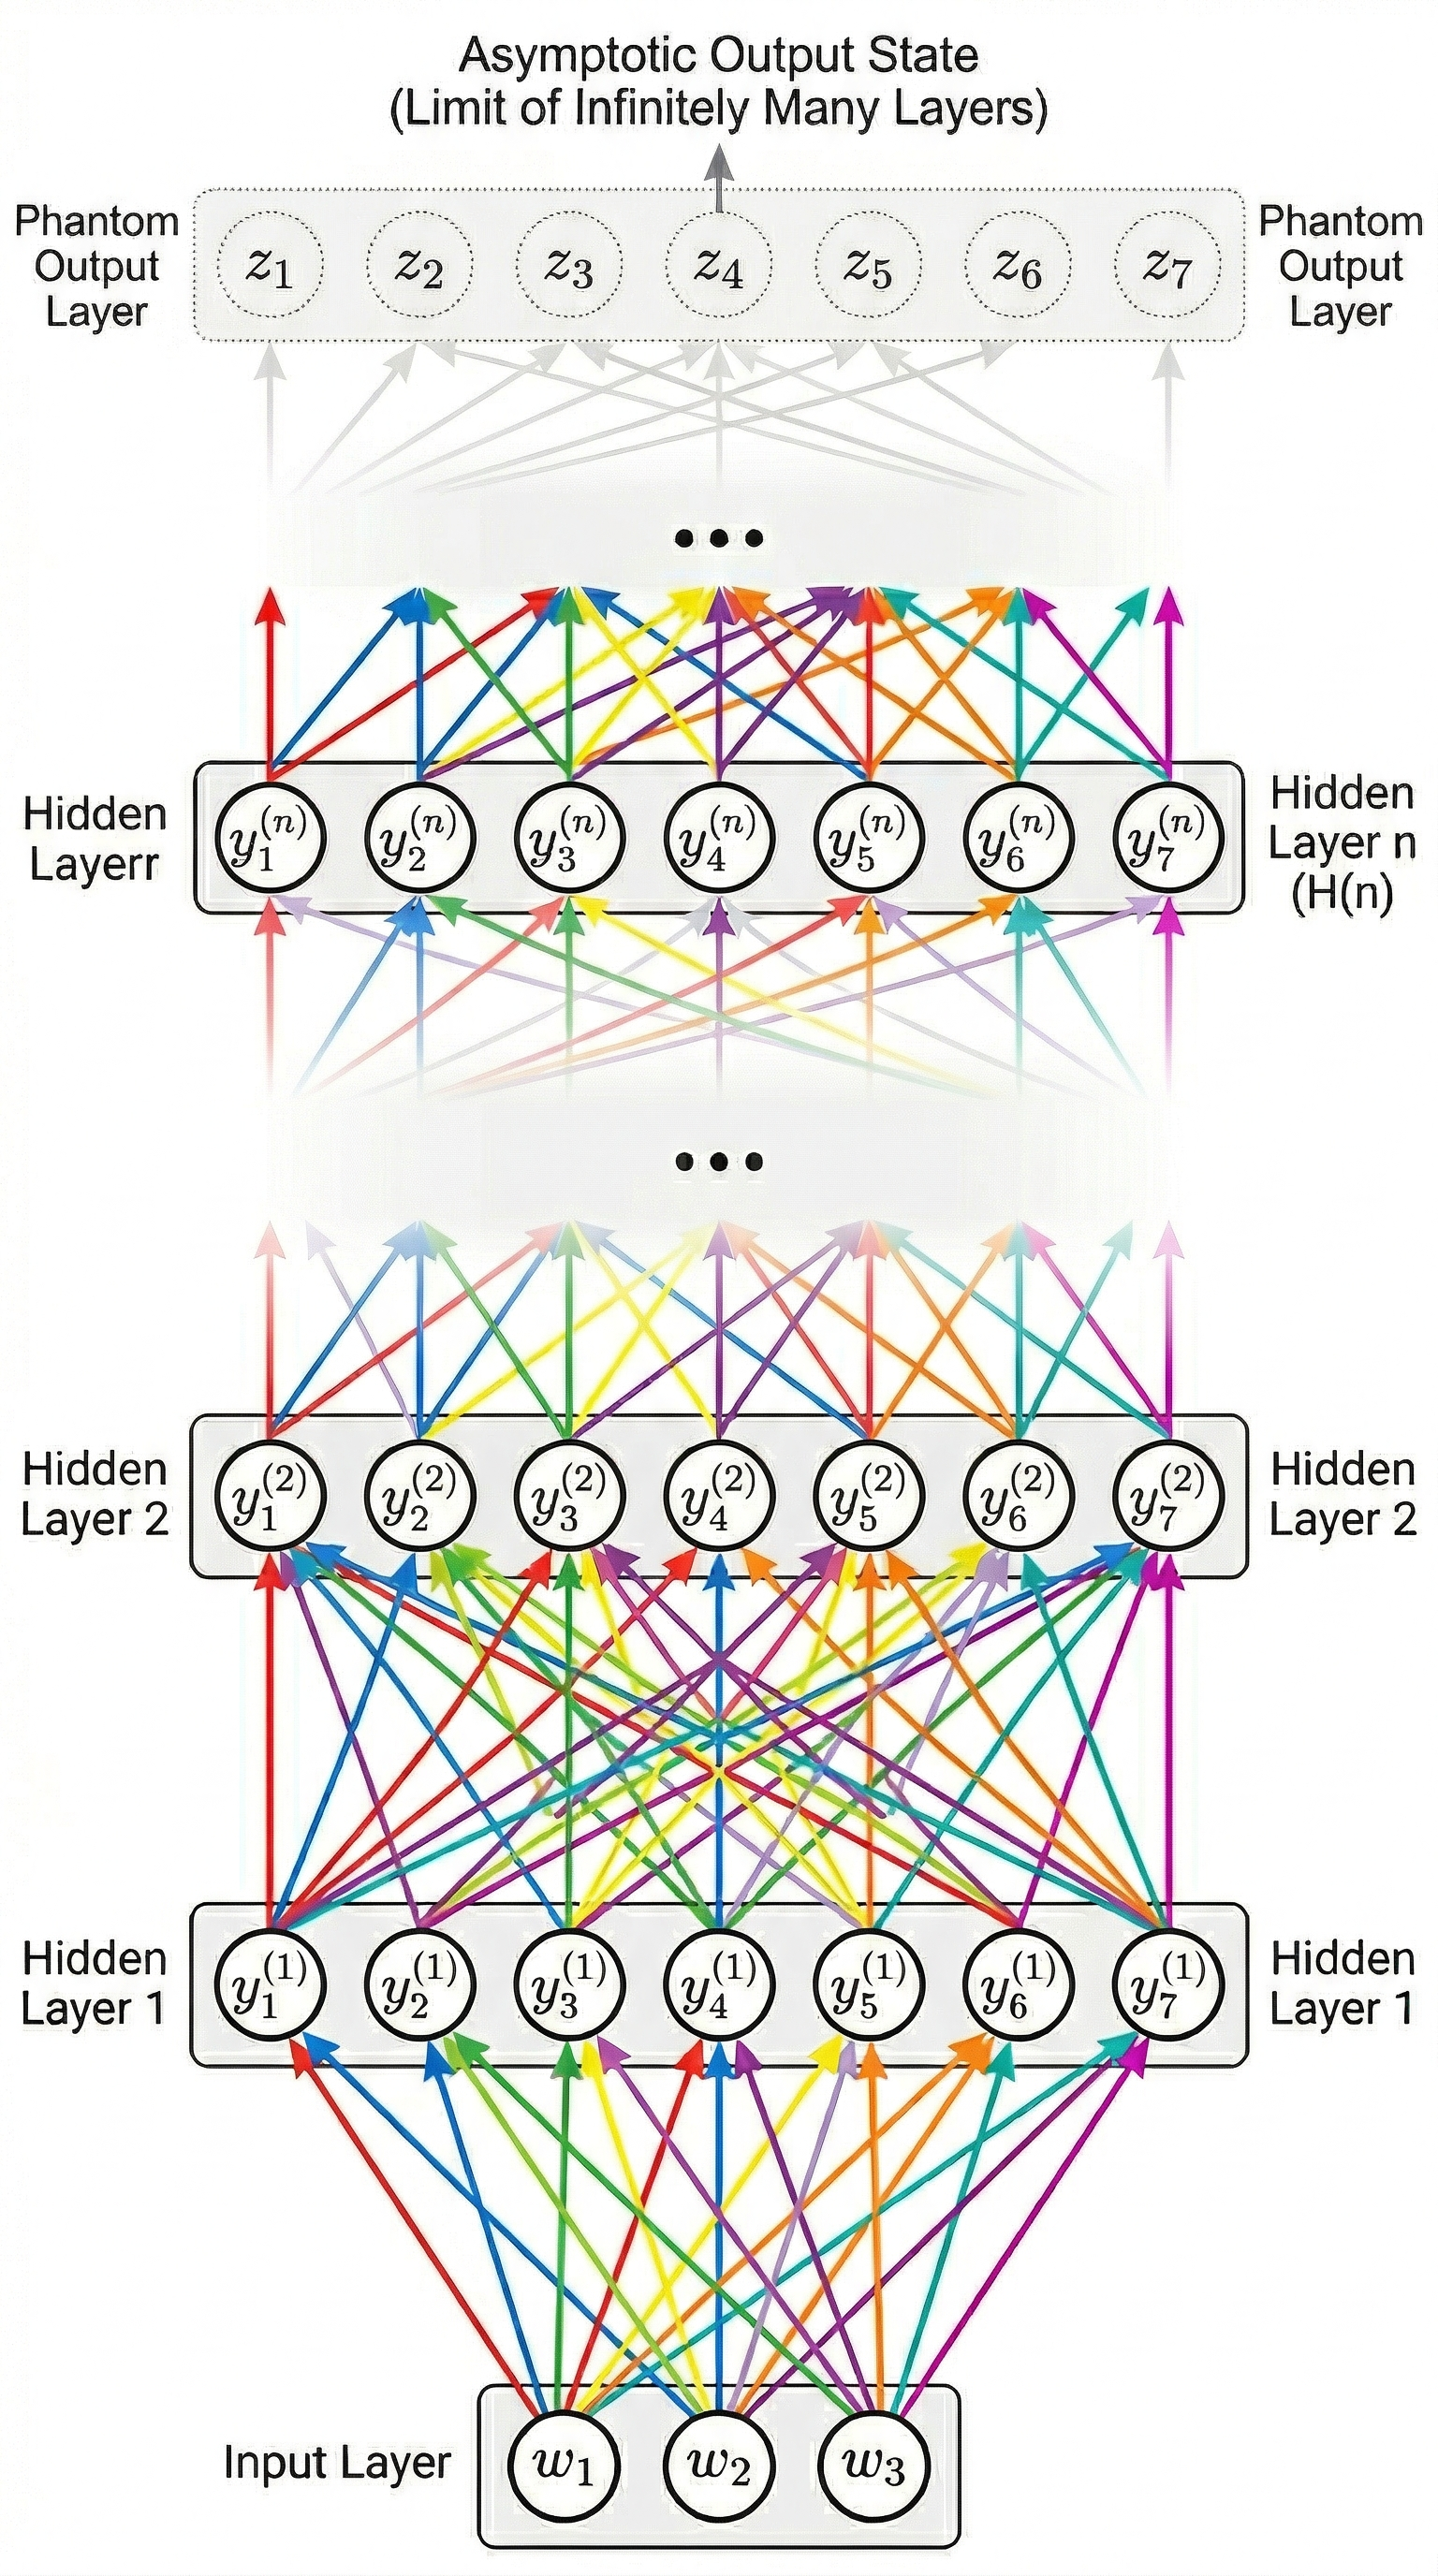
\includegraphics[scale=0.09]{../images/deep-equilibrium-labeled}
  \end{column}
  \begin{column}{0.6\textwidth}
    \begin{itemize}
    \item any map between \alert{finite}-dimensional real vector spaces whose output coordinates are continuous
    \end{itemize}
  \end{column}
\end{columns}
\end{frame}

\begin{frame}{Deep Computations: Limits of Processes}
    \begin{block}{From Finite to Infinite Depth}
    Modern computational paradigms often involve taking limits of discrete processes:
    \begin{itemize}
        \item \textbf{Deep Learning}: Depth of neural networks $d \to \infty$.
        \item \textbf{Neural ODEs}: Discretization step $\Delta t \to 0$.
        \item \textbf{Deep Equilibrium Models}: Fixed points of iterative layers.
    \end{itemize}
    \end{block}

    \pause
    
    \begin{alertblock}{The Fundamental Question}
    What is the \textbf{logical and topological complexity} of these limit maps (``deep computations'')?
    \end{alertblock}

    \vspace{0.5cm}
    \begin{center}
    Are they continuous? Measurable? Approximable?
    \end{center}
\end{frame}

\begin{frame}{The Rosetta Stone}
    Our approach bridges three distinct fields to classify these limits.
    
    \begin{center}
    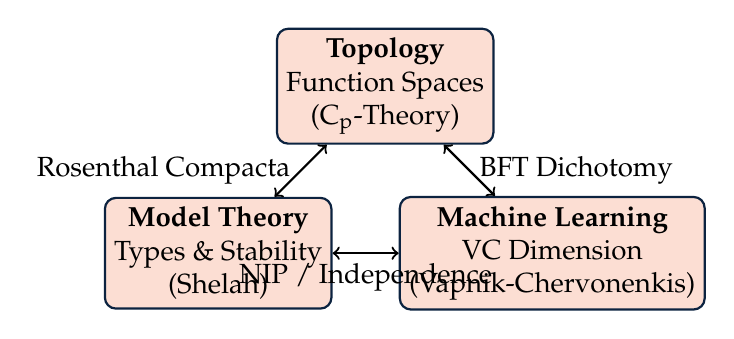
\begin{tikzpicture}[node distance=3cm, auto, thick]
        \node[draw=utsaNavy, fill=utsaOrange!20, rounded corners, align=center] (Topo) {\textbf{Topology}\\ Function Spaces \\ ($\Cp$-Theory)};
        \node[draw=utsaNavy, fill=utsaOrange!20, rounded corners, align=center] (Model) [below left of=Topo] {\textbf{Model Theory}\\ Types \& Stability \\ (Shelah)};
        \node[draw=utsaNavy, fill=utsaOrange!20, rounded corners, align=center] (Learn) [below right of=Topo] {\textbf{Machine Learning}\\ VC Dimension \\ (Vapnik-Chervonenkis)};
        
        \draw[<->] (Topo) -- node[left] {Rosenthal Compacta} (Model);
        \draw[<->] (Topo) -- node[right] {BFT Dichotomy} (Learn);
        \draw[<->] (Model) -- node[below] {NIP / Independence} (Learn);
    \end{tikzpicture}
    \end{center}
\end{frame}

%----------------------------------------------------------------------------------------
%	SECTION 2: COMPUTATION STRUCTURES
%----------------------------------------------------------------------------------------
\section{Computation Structures}

\begin{frame}{Computation States Structures (CSS)}
    We formalize a computational environment as a pair $(L, \mathcal{P})$:
    
    \begin{itemize}
        \item \textbf{States ($L$)}: The set of all possible memory states of the machine.
        \item \textbf{Features ($\mathcal{P}$)}: A family of real-valued functions $P: L \to \mathbb{R}$ (observables).
    \end{itemize}

    \begin{example}[Vector Space]
        $L = \mathbb{R}^n$, $\mathcal{P} = \{ \text{projections } \pi_1, \dots, \pi_n \}$.
    \end{example}

    \pause 

    \begin{block}{The Space of Types $\mathcal{L}$}
     Embed states into feature space: $v \mapsto (P(v))_{P \in \mathcal{P}}$. 
     The \textbf{Type Space} $\mathcal{L}$ is the topological closure of the image of $L$ in $\mathbb{R}^\mathcal{P}$.
     \begin{itemize}
         \item $\mathcal{L}$ captures ``ideal'' or ``limit'' states.
         \item Topology: Pointwise convergence (product topology).
     \end{itemize}
    \end{block}
\end{frame}

\begin{frame}{Compositional Computation Structures (CCS)}
    Add dynamics to the structure: $(L, \mathcal{P}, \Gamma)$.
    
    \begin{itemize}
        \item $\Gamma \subseteq L^L$: A semigroup of \textbf{computations} (state transitions).
        \item Closed under composition and contains identity.
    \end{itemize}
    
    \begin{block}{Deep Computations}
    The space of all computations $\Gamma$ sits inside the function space $\mathcal{L}^L$ (transforming states to types).
    
    \textbf{Deep Computations} $\overline{\Gamma}$ are the topological closure of $\Gamma$.
    \end{block}
    
    \vspace{0.2cm}
    They represent the ``limit behavior'' (e.g., the map computed by an infinitely deep network).
\end{frame}

\section{Examples}

\begin{frame}{Example 1: Newton-Raphson Dynamics}
    \textbf{Task}: Find roots of a polynomial $p(z)$ on the Riemann Sphere $\hatC$.
    \begin{itemize}
        \item \textbf{States}: $L = \hatC \cong S^2$.
        \item \textbf{Features}: Inverse stereographic coordinates $(P_1, P_2, P_3)$.
        \item \textbf{Computations $\Gamma$}: Iterates of the Newton map $N_p(z) = z - \frac{p(z)}{p'(z)}$.
    \end{itemize}

    \begin{columns}
        \column{0.5\textwidth}
        \textbf{Deep Computations}:
        Evaluated at a point $z_0$, the sequence $N_p^{(n)}(z_0)$ may:
        \begin{enumerate}
            \item Converge to a root (Basins of Attraction).
            \item Converge to a cycle.
            \item Behave chaotically (Julia Set).
        \end{enumerate}
        
        \column{0.5\textwidth}
        \centering
        \includegraphics[width=0.8\textwidth]{../images/newton_div100.png} % Assuming image exists or placeholder
        \\ \tiny{Newton Fractal for $z^3-2z+2$}
    \end{columns}
\end{frame}

\begin{frame}{Example 2: Thomae's Function (The Popcorn Function)}
    % Including this as it relates to the user's thomae.py context
    Consider limits of simple rational approximations.
    
    \begin{definition}[Thomae-like Limit]
    Let $f_n(x)$ be related to Farey sequences of order $n$.
    As $n \to \infty$, we recover Thomae's function:
    \[
    f(x) = \begin{cases} 
      1/q & \text{if } x = p/q \text{ (rational reduced)}\\
      0 & \text{if } x \text{ is irrational}
    \end{cases}
    \]
    \end{definition}
    
    \begin{itemize}
        \item \textbf{Key Insight}: The limit function is discontinuous at every rational, but continuous at every irrational.
        \item It belongs to \textbf{Baire Class 1}: Pointwise limits of continuous functions.
    \end{itemize}
\end{frame}

%----------------------------------------------------------------------------------------
%	SECTION 3: CLASSIFICATION
%----------------------------------------------------------------------------------------
\section{Classification of Deep Computations}

\begin{frame}{Baire Class 1 \& NIP}
    Deep computations arise as limits. But how wild are these limits?
    
    \begin{block}{Baire Class 1}
    Functions $f$ that are pointwise limits of continuous functions.
    \end{block}

    \begin{theorem}[Fundamental Dichotomy (BFT / NIP)]
    Let $\Delta$ be a set of computations. The following are equivalent:
    \begin{enumerate}
        \item The space of deep computations $\overline{\Delta}$ is ``tame'' (relatively compact in Baire Class 1).
        \item $\Delta$ has the \textbf{No Independence Property (NIP)}.
    \end{enumerate}
    \end{theorem}
    
    \textbf{NIP (Intuition)}: The computations cannot ``shatter'' arbitrarily large finite sets of inputs. (Related to finite VC-Dimension).
\end{frame}

\begin{frame}{The Hierarchy of Tameness}
    If a system satisfies NIP, it is tame. But there are \emph{levels} of tameness.
    We use \textbf{Todorčević’s Trichotomy} for Rosenthal Compacta to define complexity classes.

    \begin{center}
    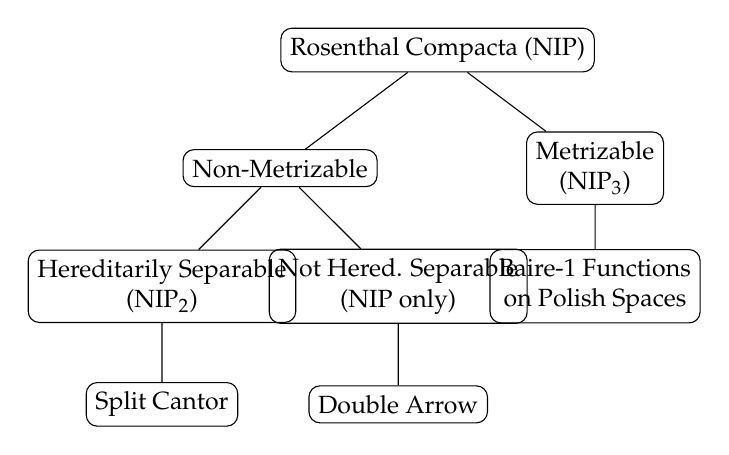
\begin{tikzpicture}[
      level 1/.style={sibling distance=4cm},
      level 2/.style={sibling distance=3cm},
      every node/.style={draw, rounded corners, align=center, font=\small}
    ]
      \node {Rosenthal Compacta (NIP)}
        child {node {Non-Metrizable}
          child {node {Hereditarily Separable \\ ($\text{NIP}_2$)}
             child {node {Split Cantor}}
          }
          child {node {Not Hered. Separable \\ ($\text{NIP}$ only)}
             child {node {Double Arrow}}
          }
        }
        child {node {Metrizable \\ ($\text{NIP}_3$)}
          child {node {Baire-1 Functions \\ on Polish Spaces}}
        };
    \end{tikzpicture}
    \end{center}

    \begin{itemize}
        \item $\NIP_3$: Metrizable (Most tame). Limits are unique and well-behaved.
        \item $\NIP_2$: Hereditarily Separable but not Metrizable.
        \item $\NIP_1$: First Countable.
    \end{itemize}
\end{frame}

\begin{frame}{The Seven Prototypes (ADK Heptachotomy)}
    Argyros, Dodos, and Kanellopoulos identified 7 minimal building blocks for these spaces. Any wilder behavior must contain one of these prototypes.
    
    \begin{columns}
        \column{0.4\textwidth}
        \begin{enumerate}
            \item $D_1$: Alexandrov compactification (Discrete)
            \item $D_2$: One-point compactification
            \item $D_3$: Split Cantor
            \item $\dots$
            \item $D_7$: Extended split Cantor
        \end{enumerate}
        
        \column{0.6\textwidth}
        \begin{alertblock}{Implication for Computing}
        If a deep computation system satisfies NIP, its asymptotic behavior is effectively approximated by a \textbf{countable discrete set} of "archetypal" limits.
        \end{alertblock}
    \end{columns}
\end{frame}

%----------------------------------------------------------------------------------------
%	SECTION 4: PROBABILISTIC VIEW
%----------------------------------------------------------------------------------------
\section{Probabilistic Computability}

\begin{frame}{Monte Carlo Computability}
    What if we relax "deterministically computable" to "computable with high probability"?
    
    \begin{definition}[Universal Monte Carlo Computable]
    A deep computation $f$ is universally Monte Carlo computable if it is $\mu$-measurable for every Radon probability measure $\mu$.
    \end{definition}

    \begin{theorem}
    If a system satisfies \textbf{NIP}, then every deep computation is universally Monte Carlo computable.
    \end{theorem}
    
    \begin{itemize}
        \item This relates to \textbf{Talagrand Stability}.
        \item "Wild" computations (IP) might not be measurable (depending on set-theoretic axioms!).
    \end{itemize}
\end{frame}

%----------------------------------------------------------------------------------------
%	SECTION 5: CONCLUSION
%----------------------------------------------------------------------------------------
\section{Conclusion}

\begin{frame}{Summary}
    We have established a framework to classify the complexity of infinite-limit computations.
    
    \vspace{0.5cm}
    
    \begin{table}[]
    \centering
    \begin{tabular}{@{}lll@{}}
    \toprule
    \textbf{Complexity} & \textbf{Topology (Rosenthal)} & \textbf{NIP Class} \\ \midrule
    Most Tame & Metrizable & $\NIP_3$ \\
    Intermediate & Hereditarily Separable & $\NIP_2$ \\
    Tame & First Countable & $\NIP_1$ \\
    Wild & Independence Property & IP \\ \bottomrule
    \end{tabular}
    \end{table}

    \vspace{0.2cm}
    \textbf{Key Takeaway}: NIP is the dividing line between physically/computationally realizable limits (Baire Class 1) and chaotic/unapproximable ones.
\end{frame}

\begin{frame}
    \centering
    \Huge Thank You!
\end{frame}

\end{document}
